\documentclass[11pt,a4paper]{article}
\usepackage[T1]{fontenc}
\usepackage[utf8]{inputenc}
\usepackage{lmodern}
\usepackage[margin=2.5cm]{geometry}
\usepackage{microtype}
\usepackage{amsmath,amssymb}
\usepackage{booktabs}
\usepackage{array}
\usepackage{graphicx}
\usepackage{tikz}
\usetikzlibrary{positioning,calc}
\usepackage[numbers,sort&compress]{natbib}
\usepackage{xcolor}
\usepackage{xurl}
\usepackage[hidelinks]{hyperref}
\usepackage{caption}
\captionsetup{font=small,labelfont=bf}
\definecolor{ours}{HTML}{E0115F}
\definecolor{refc}{HTML}{0B1F4B}
\definecolor{other}{HTML}{9FB0DC}
\definecolor{mute}{HTML}{4A5470}
\newcommand{\code}[1]{\texttt{#1}}
\setlength{\tabcolsep}{4pt}

\title{Counting passes: quantization error in a looped mixture-of-experts model, measured on Inkling 2 Mini}
\author{Daniel\\\small Master's thesis pilot, Cognitive Science}
\date{22 November 2026}

\begin{document}
\maketitle

\begin{abstract}
Inkling 2 Mini is a 26-billion-parameter mixture-of-experts model whose layers 6 to 17 run three times on the same expert weights. A quantized expert tensor therefore carries one rounding error that the model uses three times. I asked whether that error counts once, once per visit, or compounds, and whether the answer helps allocate bits in a GGUF file. I patched llama.cpp so that one pass of the loop can run on different expert weights from the other two, then changed one block of six looped layers on one pass at a time and on all three. On these documents at three passes, changing all visits costs 0.87 to 1.23 times the sum of the single-visit costs across five splits of two blocks. The ratio is much closer to one than to one third for an error that counts once or to three for perfectly aligned errors. Using the same Gaussian noise on every pass costs 1.17 to 1.22 times as much as using a fresh draw per pass. I used the measured block map to allocate bits in an 11.5\,GB file that runs fully on Apple's Metal backend. It has lower KL than each of eight other all-Metal files under 11.6\,GB that I scored. It failed the pre-registered gate against Unsloth's UD-IQ3\_XXS. The gap came mainly from the gate\_up expert encoding. Under a per-column importance metric, UD-IQ3\_XXS's encoding looks worse than mine, and under the full input second moment it looks better. Refining my codes under the full metric closed 0.93 of the gap on the selection text, 0.74 on held-out WikiText and 0.18 on reasoning traces. This is an exploratory pilot on one machine, one engine commit and one reference.
\end{abstract}

\section{Introduction}

For local use, the file size sets a budget for quantization. Every tensor competes for bits. Tools like llama.cpp's \code{llama-quantize} and the per-layer mixes that groups such as Unsloth publish treat a model as a stack of layers, each used once per token. Looped models break that assumption. In Inkling 2 Mini, the twelve core layers run three times per token, so reducing the precision of a core layer changes three visits at once.

How should an allocator price that bit? The error might count once if the loop cancels the error from earlier visits. It might count once per visit, so a looped layer costs three times a plain one. Or the visits might interact, with a joint cost above or below their sum. LoopQ identifies recursive error accumulation as a source of degradation~\citep{loopq}. Summing Hessians over loop steps gave better results than using a one-step Hessian in a recurrent-depth model~\citep{feedback}. In loops that settle, a fixed rounding error does not accumulate~\citep{tiltedbowl}. None of these studies applies a quantized expert block to one pass only and compares the result with all passes, and none works on a mixture-of-experts model in GGUF form.

In this master's thesis pilot:
\begin{itemize}
\item I patched llama.cpp so each pass of the loop can use its own expert tensors, wrote tests that fail without those patches and fixed a bug in how later passes read expert scales.
\item I tested the effect of changing one pass at a time in a looped block. I also ran a layer-split control, a Gaussian-noise control and a test on a second block. I registered each test before collecting its data.
\item I used a measured block map to choose an 11.5\,GB GGUF (``v1''). It failed the pre-registered gate and passed a narrower comparison.
\item I traced the KL gap to the gate\_up encoding and tested a code refinement that recovered most of the gap on WikiText, with a smaller gain on reasoning traces.
\end{itemize}

I copied every number below from the repository's \code{results/} directory or from the dated records in \code{CHANGELOG.md}, which scripts wrote from the run logs. None of these results is confirmatory evidence.

\section{The model and its loop}

The model is \code{thinkingmachines/Inkling-2-Mini}~\citep{inkling}. \code{llama-bench} reports 26.07\,B parameters. It has 24 layers. Each layer has 128 routed experts stored in two tensors. \code{ffn\_gate\_up\_exps} holds the fused gate and up projections, and \code{ffn\_down\_exps} holds the down projection. I call them gate\_up and down. In the release, layers 0 to 19 store their expert weights in NVFP4 and layers 20 to 23 in MXFP8.

Layers 6 to 17 form the looped core. With $P$ passes the model makes $12 + 12P$ layer visits, so the default $P = 3$ gives 48 visits from 24 layers. The model rejects $P = 1$. In the pinned llama.cpp commit, layers 0 to 5 run once, the core runs $P$ times and layers 18 to 23 run once. Passes 2 and 3 restart from the output of layer 5 and read the previous pass through small loop-control tensors. Every layer visit has its own key-value cache slot (Figure~\ref{fig:loop}). Pass 1 uses slots 6 to 17, and for pass $p \in \{2,3\}$ over core layer $l$ the slot is $24 + 12(p-2) + (l - 6)$.

I group the layers into five blocks: B1 (layers 0-5, before the loop), B2 (6-11, looped), B3 (12-17, looped), B4 (18-19, after the loop) and B5 (20-23, after the loop, MXFP8 source).

\begin{figure}[t]
\centering
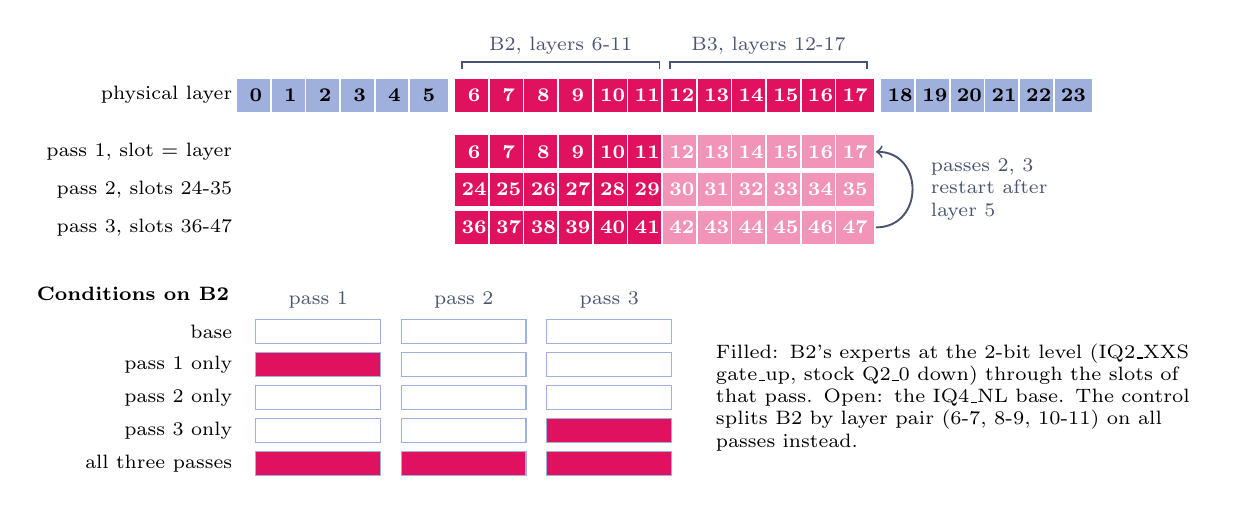
\begin{tikzpicture}[x=0.44cm,y=0.6cm,font=\scriptsize,
  box/.style={draw=white,line width=0.6pt,minimum width=0.5cm,minimum height=0.44cm,inner sep=0pt,text=white,font=\scriptsize\bfseries}]
  % physical layers
  \node[anchor=east,font=\scriptsize] at (-0.4,3) {physical layer};
  \foreach \i in {0,...,5}  {\node[box,fill=other,text=black] at (\i,3) {\i};}
  \foreach \i in {6,...,17} {\node[box,fill=ours] at (\i+0.3,3) {\i};}
  \foreach \i in {18,...,23}{\node[box,fill=other,text=black] at (\i+0.6,3) {\i};}
  % slots
  \node[anchor=east] at (-0.4,1.8) {pass 1, slot = layer};
  \node[anchor=east] at (-0.4,1.0) {pass 2, slots 24-35};
  \node[anchor=east] at (-0.4,0.2) {pass 3, slots 36-47};
  \foreach \i in {6,...,17} {
    \pgfmathtruncatemacro{\a}{\i+18}\pgfmathtruncatemacro{\b}{\i+30}
    \ifnum\i<12 \def\c{ours}\else\def\c{ours!45}\fi
    \node[box,fill=\c] at (\i+0.3,1.8) {\i};
    \node[box,fill=\c] at (\i+0.3,1.0) {\a};
    \node[box,fill=\c] at (\i+0.3,0.2) {\b};
  }
  \draw[mute,line width=0.6pt] (5.95,3.55) -- (5.95,3.7) -- (11.65,3.7) -- (11.65,3.55);
  \node[mute] at (8.8,4.05) {B2, layers 6-11};
  \draw[mute,line width=0.6pt] (11.95,3.55) -- (11.95,3.7) -- (17.65,3.7) -- (17.65,3.55);
  \node[mute] at (14.8,4.05) {B3, layers 12-17};
  \draw[->,mute,line width=0.7pt] (17.9,0.2) .. controls (19.3,0.2) and (19.3,1.8) .. (17.9,1.8);
  \node[mute,anchor=west,align=left] at (19.2,1.0) {passes 2, 3\\restart after\\layer 5};
  % conditions
  \node[anchor=west,font=\scriptsize\bfseries] at (-6.6,-1.2) {Conditions on B2};
  \foreach \row/\lab/\on in {0/base/000, 1/pass 1 only/100, 2/pass 2 only/010, 3/pass 3 only/001, 4/all three passes/111} {
    \node[anchor=east] at (-0.4,-2.0-0.7*\row) {\lab};
    \foreach \p in {1,2,3} {
      \pgfmathtruncatemacro{\bit}{mod(floor(\on/10^(3-\p)),10)}
      \ifnum\bit=1 \def\f{ours}\else\def\f{white}\fi
      \draw[fill=\f,draw=other] ({(\p-1)*4.2+0.0},{-2.0-0.7*\row-0.25}) rectangle ++(3.6,0.5);
    }
  }
  \foreach \p in {1,2,3} {\node[mute] at ({(\p-1)*4.2+1.8},-1.35) {pass \p};}
  \node[anchor=west,align=left,text width=6.2cm] at (13.0,-3.4) {Filled: B2's experts at the 2-bit level (IQ2\_XXS gate\_up, stock Q2\_0 down) through the slots of that pass. Open: the IQ4\_NL base. The control splits B2 by layer pair (6-7, 8-9, 10-11) on all passes instead.};
\end{tikzpicture}
\caption{Physical layers, cache slots and the five conditions of the per-pass test. Patch 0003 lets a slot carry its own expert tensors, so a single pass can run on different expert weights. The diagram contains no measured values.}
\label{fig:loop}
\end{figure}

Two details affected the builds. The down projection's rows are 1152 wide, which is not a multiple of 256, so \code{llama-quantize} silently replaces every 256-block type (the IQ1 to IQ3 families, Q2\_K, Q3\_K, Q4\_K) with IQ4\_NL, Q4\_0 or Q5\_0 for down, even when asked for a specific type. I read the tensor types and byte count from each built file. Unsloth-style GGUFs keep the release's NVFP4 weights together with a per-expert \code{.scale} tensor. In llama.cpp before upstream commit \code{690b87d} (21 November), passes 2 and 3 ran those experts without their scale. Patch 0001 fixed this locally and patch 0002 tests it.

\section{Instrument and setup}

\paragraph{Engine.} I used llama.cpp \code{29b52d3} (b12600) with seven patches, built for Release with Metal, on one Apple M5 Pro with 48\,GB of memory. I ran one heavy process at a time. Patches 0003 and 0005 let a cache slot carry its own expert tensors. Patch 0007 speeds up the BF16 conversion of packed expert tensors. Patches 0002, 0004 and 0006 are tests. Twelve loop checks pass. Four match with nmse 0, and the largest nmse among the rest is 7.0e-09. Stock upstream llama.cpp (\code{c661033}, no patches) gives v1 the same scores as the patched build on T1 (KL 0.026856, top-1 93.139\%).

\paragraph{Reference and metric.} I converted the release to a Q8\_0 GGUF for the reference and scored it at the same $P$ as the file under test. Using a different pass count would include the effect of changing the loop in the KL measurement. The metrics are mean KL divergence and top-1 agreement against that reference from \code{llama-perplexity --kl-divergence}. The text is fixed, so scoring involves no sampling. Intervals are 95\% percentile bootstraps over chunks with 10,000 resamples and seed 0, paired whenever two files are compared.

\paragraph{Data.} I used S for every selection decision. I held out T1 and T2 and scored them only after fixing the candidate (Table~\ref{tab:data}). T2 consists of reasoning traces generated by the reference at $P = 3$ from 40 GSM8K training questions~\citep{gsm8k} with low effort, temperature 0 and a 2,048-token cap. The traces total 10,628 completion tokens. None hit the cap, and I generated them all before building any candidate. S and T1 come from the WikiText-2 test split~\citep{wikitext}. None of the sets shares an exact 13-word sequence with the calibration text behind the importance matrix.

\begin{table}[t]
\centering\small
\caption{Evaluation sets. Overlap counts exact word 13-grams shared with bartowski's v6 calibration text, the source of the importance matrix.}
\label{tab:data}
\begin{tabular}{llll}
\toprule
Set & Content & Size & Shared 13-grams \\
\midrule
S & WikiText-2 test, 16 chunks of 4,096 tokens & 65,792 tokens & 0 of 43,499 \\
T1 & WikiText-2 test, next 16 chunks of 4,096 tokens & 65,792 tokens & 0 of 42,630 \\
T2 & reasoning traces, 5 chunks of 2,048 tokens & 40 prompts & n/a \\
\bottomrule
\end{tabular}
\end{table}

\paragraph{Registration.} The pre-registration of 20 November fixed the hypotheses, the data splits, the stop rules and the release gate. I recorded each later change in a dated entry in \code{CHANGELOG.md} before collecting the data it governs. Where I registered a decision rule, I report its outcome, including failures.

\paragraph{Floors.} The reference scored against itself gives KL 0.00000 and top-1 100.00\%. My IQ4\_NL build gives KL 0.01619 on S, inside the registered stop band of 0.005 to 0.02.

\section{The block map}

Before testing individual passes, I measured the KL cost of quantizing each block. In each run I changed one block's expert tensors to a lower-bit level and kept everything else as in the reference (Table~\ref{tab:map}). The 2-bit level is IQ2\_XXS gate\_up with Q2\_0 down. The 3-bit level is IQ3\_XXS gate\_up with IQ4\_NL down. I built the variants by copying tensors byte for byte between pre-quantized pool files, which reproduces \code{llama-quantize}'s output for the same types and importance matrix.

\begin{table}[t]
\centering\footnotesize
\caption{Block map. KL on S at $P = 3$ with one block's experts changed and the rest as in the Q8\_0 reference. Columns give gate\_up / down types. ``Q2\_0 (mine)'' uses the importance-weighted Q2\_0 encoder of Section~\ref{sec:side}.}
\label{tab:map}
\begin{tabular}{llrrrrr}
\toprule
Block & Layers & \shortstack{IQ2\_XXS\\Q2\_0} & \shortstack{IQ2\_XXS\\IQ4\_NL} & \shortstack{IQ2\_S\\IQ4\_NL} & \shortstack{IQ3\_XXS\\Q2\_0 (mine)} & \shortstack{IQ3\_XXS\\IQ4\_NL} \\
\midrule
B1 & 0-5 & 0.02789 & 0.00937 & 0.00693 & 0.01201 & 0.00529 \\
B2 & 6-11, looped & 0.06235 & 0.01881 & 0.01240 & 0.02089 & 0.00822 \\
B3 & 12-17, looped & 0.08519 & 0.02188 & 0.01317 & 0.02279 & 0.00768 \\
B4 & 18-19 & 0.03593 & 0.00731 & 0.00403 & 0.00927 & 0.00233 \\
B5 & 20-23, MXFP8 & 0.06675 & 0.01670 & 0.00876 & 0.01655 & 0.00469 \\
\bottomrule
\end{tabular}
\end{table}

At the 2-bit level, B4 and B5 cost more per layer than the looped blocks. KL per layer is 0.0180 for B4 and 0.0167 for B5, against 0.0104 for B2 and 0.0142 for B3. At the 3-bit level, B2 costs the most per layer at 0.00137. A looped layer runs three times, but its rank depends on the quantization level. The map changes a looped block on all passes at once, so it cannot separate their costs. The block KLs also differ from the KL of a joint change. The five 2-bit block KLs sum to 0.2781, against 0.3046 for the uniform 2-bit build (ratio 1.10), while at 3 bits the sum is 0.0282 against 0.0221 (0.78). Non-expert tensors at Q6\_K with reference experts cost 0.00353.

I also scored the uniform builds at $P = 2$ and $P = 4$, each against the reference at its own $P$. KL is lowest at $P = 3$ for both levels (2-bit values of 0.4285, 0.3046 and 0.3365, and 3-bit values of 0.0456, 0.0221 and 0.0327). The model was tuned at $P = 3$, so this comparison gives no causal evidence about how error accumulates.

\section{Do the passes add up?}
\label{sec:perpass}

\subsection{Design}

In the per-pass test I change block B2 to the 2-bit level on pass 1 only, pass 2 only, pass 3 only, or all three, using the slots of Figure~\ref{fig:loop}. I use the IQ4\_NL build as the base. A Q8\_0 base would need Q8\_0 copies of layers 6 to 11 for the untouched passes, about 36 to 41\,GB, above the pilot's memory limit. At this level the mean relative weight error against the base is 0.5292 on down and 0.1288 on gate\_up. Two registered checks came first. A no-op splice reproduced the base logits byte for byte, and switching all three passes through slot tensors reproduced an ordinary build with the same tensors.

Let $d_k$ be the change in log-probabilities, over all tokens and vocabulary entries, when only pass $k$ is changed, and $d_{\text{all}}$ the change when all three are. If the passes added up exactly, $d_{\text{all}} = d_1 + d_2 + d_3$. I measure the departure with the residual share and the norm ratio
\begin{equation}
r = \frac{\lVert d_{\text{all}} - \sum_k d_k \rVert}{\lVert d_{\text{all}} \rVert}, \qquad
\rho = \frac{\lVert d_{\text{all}} \rVert}{\lVert \sum_k d_k \rVert},
\end{equation}
which are 0 and 1 for exact additivity. The norm is the Fisher norm under the base distribution. For each token $t$ with base probabilities $p_t$, the squared norm is the variance of the change under $p_t$, summed over tokens, so that KL is half the squared norm to second order. I also report the ratio of KLs, $\mathrm{KL}_{\text{all}} / \sum_k \mathrm{KL}_k$. To second order it separates the three answers from the introduction. If the error counts once, changing all visits costs about what one visit costs and the ratio is about $1/3$. If each visit adds an independent error, the ratio is about 1. If the three visit errors were identical and aligned, $\lVert 3d \rVert^2 = 9 \lVert d \rVert^2$ against $3 \lVert d \rVert^2$, and the ratio is about 3.

Any split of a nonlinear model can leave a residual. The registered control (Addendum F) splits the same block by layer pair, with the 2-bit change on layers 6-7, 8-9 or 10-11, each on all passes. Those three parts share no weights. The registered rule requires the pass split and the layer split to differ beyond both 95\% intervals for both $r$ and $\rho$. In Addendum H I registered further tests before collecting their data. I repeated the control at 3 bits, ran B3 and replaced quantization with Gaussian noise of the same relative error. Following the linearity analysis of \citet{linearity}, I used either the same draw on every pass (tied) or draw $k$ on pass $k$ (independent).

\subsection{Results}

\begin{table}[t]
\centering\footnotesize
\caption{Additivity statistics on S at $P = 3$, against the IQ4\_NL base, Fisher norm, with 95\% chunk intervals. For entries marked ``point only'', the per-chunk logits were deleted before the per-chunk KLs were kept.}
\label{tab:perpass}
\begin{tabular}{lllll}
\toprule
Split & Block, level & $r$ & $\rho$ & KL all / sum \\
\midrule
pass & B2, 2-bit & 0.675 [0.657, 0.693] & 0.841 [0.829, 0.855] & 1.135 [1.112, 1.162] \\
layer pair (control) & B2, 2-bit & 0.838 [0.822, 0.855] & 0.759 [0.748, 0.770] & 0.888 (point only) \\
pass & B2, 3-bit gate\_up & 0.748 [0.732, 0.761] & 0.788 [0.780, 0.794] & 0.875 (point only) \\
layer pair (control) & B2, 3-bit gate\_up & 1.108 [1.074, 1.145] & 0.640 [0.627, 0.652] & 0.616 [0.591, 0.638] \\
pass & B3, 2-bit & 0.539 [0.526, 0.553] & 0.906 [0.897, 0.915] & 1.226 [1.209, 1.244] \\
pass, tied noise & B2 & 0.680 [0.660, 0.702] & 0.836 [0.825, 0.847] & 1.141 [1.119, 1.162] \\
pass, independent noise & B2 & 0.723 [0.709, 0.736] & 0.807 [0.798, 0.817] & 0.953 [0.934, 0.971] \\
\bottomrule
\end{tabular}
\end{table}

\begin{figure}[t]
\centering
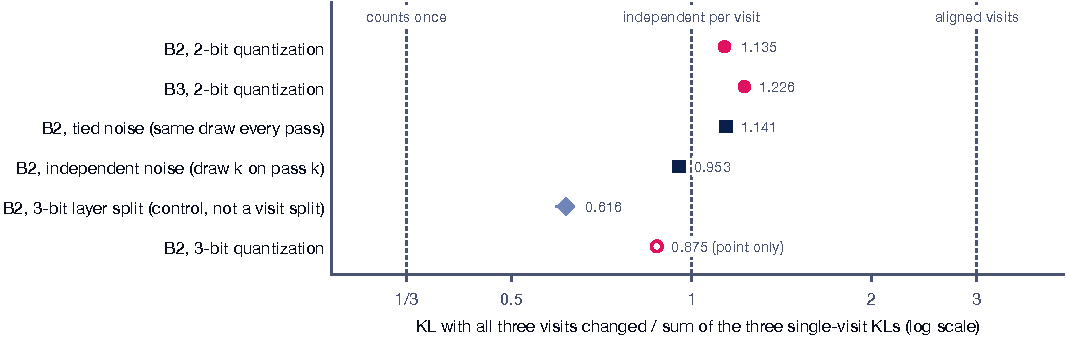
\includegraphics[width=\linewidth]{fig/additivity.pdf}
\caption{KL with all three visits changed, divided by the sum of the three single-visit KLs, for each split on S at $P = 3$. Dashed lines mark the second-order values for an error that counts once (1/3), independent errors per visit (1) and three identical, aligned visit errors (3). Intervals are 95\% paired chunk bootstraps and are mostly narrower than the markers. The open marker has no interval.}
\label{fig:additivity}
\end{figure}

\paragraph{Pass split and layer split.} At 2 bits on B2, $r = 0.675$, so the sum of the three single-pass changes leaves a large residual (Table~\ref{tab:perpass}). The layer-split control leaves an even larger residual, $r = 0.838$, and the intervals for both $r$ and $\rho$ do not overlap, so the registered rule is met. Splitting the change across passes on shared weights is closer to additive than splitting it across layers. The same rule is met at 3 bits ($r$ of 0.748 against 1.108, with the larger $r$ in the layer split in 16 of 16 chunks). The residual share rises from 0.675 to 0.748 even though the 3-bit all-pass KL is 0.00809, about 7.7 times smaller than the 2-bit value of 0.06198.

\paragraph{The error counts about once per visit.} Across the five visit splits with per-chunk data, the KL ratio runs from 0.953 to 1.226, and the 3-bit point estimate is 0.875 (Figure~\ref{fig:additivity}). All are closer to 1 than to the 1/3 that ``counts once'' predicts or to the aligned value of 3, although the B3 interval excludes 1. The norm of the all-pass logit change is smaller than the norm of the sum of the single-pass changes ($\rho$ of 0.841 on B2 and 0.906 on B3). I see little compounding within three passes.

\paragraph{Tied noise costs more.} The noise conditions let me compare tied and independent noise at nearly equal single-pass cost. The single-pass KLs of the tied and independent draws sum to almost the same value (0.05566 and 0.05572), yet tied noise costs more when applied on all passes. Over every pairing of three tied and three independent draws, the ratio KL(tied) / KL(independent) lies between 1.167 and 1.223, with the lowest lower bound at 1.146, so the registered rule ``tied costs more'' is met. Tied noise behaves like the quantization error of the same size (KL ratio 1.141 against 1.135, $r$ of 0.680 against 0.675). Independent noise is slightly sub-additive (0.953, interval excluding 1) and fails the registered criterion for ``about additive''. The pairwise Fisher cosines between single-pass changes are 0.320, 0.362 and 0.138 for tied noise against 0.267, 0.216 and 0.111 for independent noise (passes 1-2, 2-3 and 1-3). The single-pass changes align more closely under tied noise.

\paragraph{The costliest visit depends on block and level.} On B2 at 2 bits the single-pass KLs are 0.01885, 0.01983 and 0.01591 for passes 1 to 3. On B3 they are 0.01661, 0.02069 and 0.03244, and the last pass carries most of the all-pass change (share 0.629 against 0.514 on B2). At 3 bits on B2, pass 1 is the costliest (0.004671, against 0.002805 and 0.001771). One fixed weight per visit will not fit all of these.

\subsection{What this means for allocation}

For this setup, I would price a bit in a looped layer roughly per visit, with a surcharge of about a fifth for shared weights and a share for each pass that depends on the block. The test gives little support to pricing a bit once, as a plain transformer allocator implicitly does, or to pricing the error as compounding. The test leaves open why the residual is large. Changes in the router's expert choices and smooth nonlinearity could both contribute. A route-replay run that forces the base's expert choices on every visit would separate them. I noted that test but did not run it. I made three analysis choices that differ from the registered plan: the Fisher norm as the primary norm, a 10-nat head for the Euclidean check (the logits files floor log-probabilities 16 nats below the maximum, which makes the registered full-vocabulary form uncomputable), and a ratio of sums over tokens instead of a per-token ratio. I fixed them in code before the per-pass logits existed and recorded the deviations in the change log. The Euclidean norm on the head and the full-vocabulary norm with floored entries give the same verdict.

\section{A release candidate and a failed gate}
\label{sec:release}

I also asked whether a block-wise allocation chosen from the map could give lower KL than a public 3-bit file at the same or smaller size. The byte limit was the size of Unsloth's UD-IQ3\_XXS~\citep{unslothgguf}, 11,663,310,784 bytes. I restricted the candidate to types the pinned Metal backend can multiply. UD-IQ3\_XXS keeps the release's NVFP4 down projections in 20 expert tensors that run on the CPU on a Mac.

\paragraph{Selection.} The allocator added per-projection changes from the map and proposed four allocations under the limit, each differing from the earlier picks in at least two of its eleven choices. I built and scored all four on S and chose the file with the lowest measured KL (Table~\ref{tab:sel}). The allocator overpredicted KL for all four (measured over predicted 0.73 to 0.81) and ranked them wrongly. Its first choice, sel-0, had the highest measured KL. The map's block KLs are only a rough guide to a combined build because the block KLs do not add.

\begin{table}[t]
\centering\footnotesize
\caption{Selection on S. Allocation as gate\_up / down per block. ``Q2\_0o'' is my Q2\_0 encoder. I took the byte counts from the built files.}
\label{tab:sel}
\begin{tabular}{>{\raggedright\arraybackslash}p{1.3cm}>{\raggedright\arraybackslash}p{5.6cm}lrrr}
\toprule
Pick & Allocation & Non-expert & Predicted & Measured & Bytes \\
\midrule
sel-0 & B1 IQ2\_XXS/Q2\_0o, B2-B5 IQ3\_XXS/IQ4\_NL & Q8\_0 & 0.03900 & 0.03145 & 11,576,346,656 \\
sel-1 & B1 IQ2\_XXS/IQ4\_NL, B2-B4 IQ3\_XXS/IQ4\_NL, B5 IQ2\_S/IQ4\_NL & Q6\_K & 0.03989 & 0.02963 & 11,598,989,600 \\
sel-2 (v1) & B1 IQ2\_XXS/IQ4\_NL, B2 IQ2\_S/IQ4\_NL, B3-B5 IQ3\_XXS/IQ4\_NL & Q6\_K & 0.04001 & 0.02931 & 11,514,054,944 \\
sel-3 & B1 IQ2\_S/Q2\_0o, B2-B5 IQ3\_XXS/IQ4\_NL & Q6\_K & 0.04011 & 0.02945 & 11,450,353,952 \\
\bottomrule
\end{tabular}
\end{table}

\paragraph{The gate.} The registered gate required lower paired KL than both UD-IQ3\_XXS and the plain IQ3\_XXS build on T1 and T2, with the 95\% interval excluding zero and top-1 no worse. The candidate had higher KL than UD-IQ3\_XXS on every chunk of both sets (Table~\ref{tab:gate}). The gate result was FAIL. I made no release under that gate and did not repeat selection after seeing T1 and T2. The plain IQ3\_XXS build exceeded the byte limit (11,747,211,680 bytes), and the candidate had lower KL than it on every chunk of both sets.

\begin{table}[t]
\centering\footnotesize
\caption{The release gate. Differences are candidate minus baseline. Negative values favour the candidate. ``Worse'' counts chunks where the candidate has the higher KL. Top-1 agreement is in percent, candidate / baseline.}
\label{tab:gate}
\begin{tabular}{llrrlrl}
\toprule
Set & Baseline & KL cand & KL base & Difference [95\% CI] & Worse & Top-1 \\
\midrule
T1 & UD-IQ3\_XXS & 0.02686 & 0.01939 & +0.00747 [+0.00654, +0.00845] & 16 of 16 & 93.14 / 94.42 \\
T1 & stock IQ3\_XXS & 0.02686 & 0.05421 & -0.02735 [-0.02938, -0.02537] & 0 of 16 & 93.14 / 90.32 \\
T2 & UD-IQ3\_XXS & 0.01942 & 0.01361 & +0.00581 [+0.00513, +0.00673] & 5 of 5 & 95.29 / 95.95 \\
T2 & stock IQ3\_XXS & 0.01942 & 0.04622 & -0.02680 [-0.02912, -0.02407] & 0 of 5 & 95.29 / 92.67 \\
\bottomrule
\end{tabular}
\end{table}

\paragraph{Post hoc comparison.} After the FAIL, I registered a rule for a narrower comparison before scoring any files for it. Is the candidate closer to the reference than every GGUF under the limit whose expert tensors all run on Metal? I searched Hugging Face for unmodified-weight Inkling 2 Mini files from 9.0 to 11.6\,GB and read the types from each file's header. The comparison covered eight such files. The candidate has lower KL than each of them on T1 and T2, with all 16 paired intervals below zero (Figure~\ref{fig:comparison}). I did not score two lower-bit files from makers already in the set (bartowski IQ2\_XXS, AtomicChat AD-IQ2\_XXS). This post hoc comparison does not change the FAIL.

\begin{figure}[t]
\centering
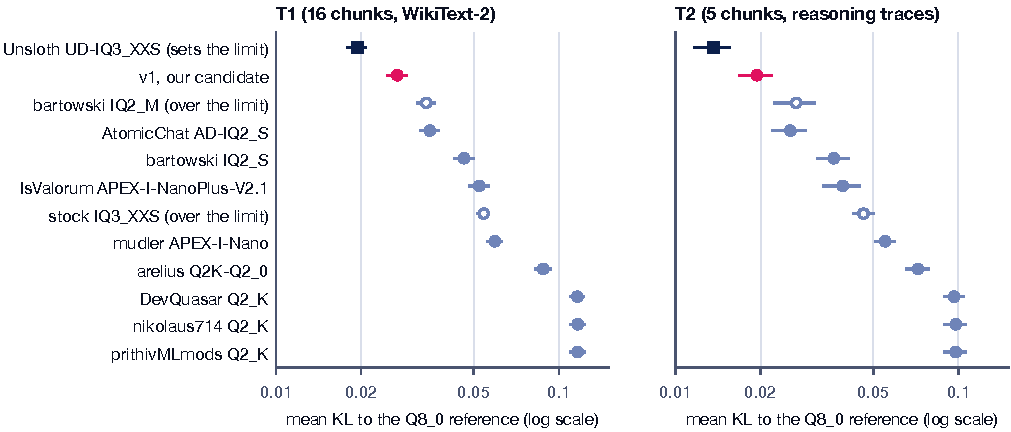
\includegraphics[width=\linewidth]{fig/comparison.pdf}
\caption{Mean KL to the Q8\_0 reference on T1 and T2 for the candidate (v1), UD-IQ3\_XXS and the all-Metal files. Open markers show files over the 11,663,310,784-byte limit for context. Intervals are unpaired 95\% chunk bootstraps of each mean. The comparisons in the text use paired differences. prithivMLmods and nikolaus714 Q2\_K score identically.}
\label{fig:comparison}
\end{figure}

\paragraph{Speed.} I benchmarked on the M5 Pro with \code{29b52d3} plus my patches, which add no kernels, using \code{llama-bench -ngl 99 -p 512 -n 128 -r 3}. The six files whose expert tensors all run on Metal ran at about the same speed, 224.41 to 235.78 tokens/s for 512-token prompts and 18.34 to 20.54 tokens/s for generation. UD-IQ3\_XXS, with 20 expert tensors on the CPU, measured 68.06 and 10.87 tokens/s. The candidate was 3.30 times as fast on prompts and 1.75 times as fast in generation. With 16K tokens already in the context the gap narrows to about 2.1 and 1.46 times. Peak memory for the candidate's process was 13.9\,GB with the context filled to 16K tokens. This speed comparison applies to stock llama.cpp. Unsloth's own prebuild includes Metal NVFP4 kernels~\citep{unslothpr}, so its NVFP4 tensors load on the GPU. I did not benchmark that build.

\paragraph{Stability.} The candidate and the reference passed all the registered stability checks. Neither showed degenerate repetition in ten 2,000-token generations at temperature 1.0. Both found a planted fact in a 16,359-token prompt, made 5 of 5 valid tool calls, gave acceptable replies in both non-English cases and got 30 of 30 GSM8K smoke-test items correct without hitting the cap. Thirty items give no accuracy estimate. The candidate is public as \code{Me-Daniel/Inkling-2-Mini-Metal-GGUF}~\citep{release}, and its card states the FAIL first.

\section{Where UD-IQ3\_XXS's lead comes from}
\label{sec:diagnosis}

To investigate the KL gap of 0.0075 on T1, I swapped tensor groups between the two files and scored the results on S. I registered the decision rule for each swap before running it. Table~\ref{tab:swap} gives the paired contrasts.

\begin{table}[t]
\centering\small
\caption{Swap diagnostics on S. Each row gives the paired KL drop from the named replacement. Positive values mean the replacement lowers KL.}
\label{tab:swap}
\begin{tabular}{lr}
\toprule
Replacement & KL drop [95\% CI] \\
\midrule
v1 with UD's NVFP4 down (layers 0-19) & +0.00118 [+0.00063, +0.00171] \\
v1 with UD's non-expert tensors & -0.00010 [-0.00058, +0.00038] \\
v1 with UD's gate\_up experts (types and encoded values) & +0.00810 [+0.00743, +0.00874] \\
v1 with my own gate\_up encoding at UD's per-layer types & +0.00214 [+0.00144, +0.00285] \\
UD's gate\_up encoding in place of mine, at UD's types & +0.00596 [+0.00524, +0.00670] \\
\bottomrule
\end{tabular}
\end{table}

\paragraph{The gate\_up encoding.} UD's gate\_up tensors alone recover 0.00810, slightly more than the 0.00782 that UD's full layout recovers at equal down. The NVFP4 down format accounts for a smaller, consistent KL reduction. The non-expert swap gives no measurable change. I first thought UD's bit allocation explained the gap, since it gives more bits to layers 1-5 and 9-11 and fewer to 12 and 18. Quantizing with my encoder at UD's exact per-layer types recovers only 0.00214, while UD's encoded values at the same types recover 0.00596 more. Most of the gain comes from the choice of codes.

\paragraph{Conversion and importance matrix checks.} I checked the inputs on the CPU. My BF16 conversion equals an independent NVFP4 decode of the release in every one of 127,401,984 checked elements, and UD's NVFP4 down times its \code{.scale} equals the release exactly. The ggml-org importance matrix I used is expert-indexed and sums all three visits of a looped layer (the ratio of looped to non-looped totals is exactly 3.0000). An importance matrix from 300 chunks of WikiText-2 training text, the domain of S, recovered 0.00055 [0.00008, 0.00099] of the encoding gap. Four times as much of the same text added +0.00019 [-0.00020, +0.00060], an interval that includes zero. The changes from other sources tried in a companion project were also near zero. The per-column importance inputs I could build closed at most about an eighth of UD's lead.

\paragraph{Diagonal and full Gram metrics.} At the same type, UD's gate\_up is further from the BF16 weights than mine under the importance-weighted diagonal metric, yet it gives much lower KL. A diagonal metric cannot see correlations between input columns. With $\Delta W$ the dequantized minus the BF16 weights of one expert and $G = \sum x x^\top$ the expert's input Gram matrix, I compared the full error $\operatorname{tr}(\Delta W G \Delta W^\top) / \operatorname{tr}(W G W^\top)$ with its diagonal version, which keeps only $\operatorname{diag}(G)$. I estimated the Gram over 100 chunks of WikiText-2 training text and pooled the inputs over all visits. In both layers tested, UD has lower error under the full Gram in 128 of 128 experts and higher error under the diagonal in 128 of 128 (Table~\ref{tab:gram}). Most of UD's lead lies along the experts' mean input. The term $n_e \lVert \Delta W m_e \rVert^2$, with $m_e$ the mean input of expert $e$ over its $n_e$ tokens, is five times smaller for UD than for my encoding in layer 6. The mean input carries about a fifth of the input energy (0.209 in layer 6, 0.190 in layer 20) and is spread over many columns. A per-column weight misses how the errors add up along that direction.

\begin{table}[t]
\centering\small
\caption{gate\_up error under the input Gram, count-weighted over 128 experts. My encoding uses \code{llama-quantize} at the same types as UD-IQ3\_XXS.}
\label{tab:gram}
\begin{tabular}{lrrrr}
\toprule
& \multicolumn{2}{c}{Layer 6 (IQ2\_S)} & \multicolumn{2}{c}{Layer 20 (IQ3\_XXS)} \\
Metric & Mine & UD & Mine & UD \\
\midrule
full Gram & 0.03487 & 0.02252 & 0.02472 & 0.02047 \\
diagonal only & 0.06207 & 0.06609 & 0.03300 & 0.03542 \\
bias (mean-input) part & 0.00643 & 0.00128 & 0.00419 & 0.00170 \\
rest & 0.02844 & 0.02124 & 0.02053 & 0.01877 \\
\bottomrule
\end{tabular}
\end{table}

\paragraph{Attenuation check.} In a companion project on the same model, rescaling blocks using the mean input lowered the per-layer error but raised KL on S by 0.072 because it shrank each expert's output. The gain $\langle q, w \rangle / \langle w, w \rangle$ fell from 0.944 to 0.793. Over 48 layer visits a small shrinkage on every visit adds up. I checked for this in v1. Its gains are about 0.996 for down and 0.97 to 1.00 for gate\_up, with gate\_up energy above 1. Rescaling every expert row to gain 1 changed KL on S by -0.00034 [-0.00068, +0.00003], an interval that includes zero. I found no evidence that attenuation explains v1's KL gap. I still needed to guard against a lower weight error obtained by shrinking expert outputs.

\section{Refining codes under the full Gram}
\label{sec:refine}

UD's codes have lower error under the full Gram, so I tested whether choosing my codes under the same objective could close part of the gap without changing format, types or bytes. I wrote the search in \code{scripts/refine-codes.py}. It starts from \code{llama-quantize}'s gate\_up at UD's types, keeps every block's fp16 scale and sub-block scales, and changes only grid indices and signs. Per expert, with $E$ the error matrix and $H = G + 0.1\,\operatorname{Diag}(G)$, it minimizes $\operatorname{tr}(E H E^\top)$ by sweeping groups of 8 (IQ2\_S) or 4 (IQ3\_XXS) weights. For each group it uses exact incremental updates to find the representable code that lowers the objective most, if any does. I registered three safeguards before scoring any refined build. Experts with fewer than 2,304 Gram tokens (fewer tokens than input dimensions) keep their codes. I fixed the shrinkage toward the diagonal at 0.1 without tuning it. The search accepts a move only if the row's output gain $q_r H w_r^\top / w_r H w_r^\top$ stays at or above its starting value. MACaQ~\citep{macaq} describes the same core idea in an appendix of its 11 November version. It refines llama.cpp IQ3 codes in a Hessian metric with fixed scales and tests the method on dense Qwen3 models. I found it only after building mine. I use per-expert Grams pooled over the three loop visits, include a sign search for IQ2\_S and constrain the output gain. I also measure the effect on text from another domain.

\paragraph{Pilot.} On layers 9 to 11, where UD's gate\_up was worth 0.00100 [0.00055, 0.00140] on S, the refined tensors recovered 0.00111 [0.00067, 0.00156], a share of 1.11 against a registered pass mark of one half. The KL difference between my refined tensors and UD's tensors for those layers was -0.00011 [-0.00038, +0.00017]. On these three layers, my refined tensors and UD's are level within that interval. Restoring each row to the original plain gain did not help (share 0.99), so I kept the output-gain floor.

\paragraph{All layers.} v2r applies the refinement to all 22 gate\_up layers the refiner supports. Layers 0 and 4 keep \code{llama-quantize}'s bytes. The file has 11,566,703,648 bytes, the same as its unrefined base v2a, and every expert tensor runs on Metal. Its generation speed matches v1 within the benchmark's run-to-run spread.

\begin{table}[t]
\centering\footnotesize
\caption{v2r against its unrefined base v2a and UD-IQ3\_XXS. Differences are paired over chunks. I had seen all three sets before scoring v2r.}
\label{tab:v2r}
\begin{tabular}{lrrrllr}
\toprule
Set & v2r & v2a & UD & v2r minus v2a & v2r minus UD & Gap closed \\
\midrule
S & 0.02102 & 0.02779 & 0.02050 & -0.00677 [-0.00758, -0.00610] & +0.00052 [-0.00030, +0.00133] & 0.93 \\
T1 & 0.02077 & 0.02462 & 0.01939 & -0.00385 [-0.00470, -0.00298] & +0.00138 [+0.00059, +0.00218] & 0.74 \\
T2 & 0.01829 & 0.01929 & 0.01361 & -0.00100 [-0.00186, +0.00009] & +0.00468 [+0.00333, +0.00626] & 0.18 \\
\bottomrule
\end{tabular}
\end{table}

\begin{figure}[t]
\centering
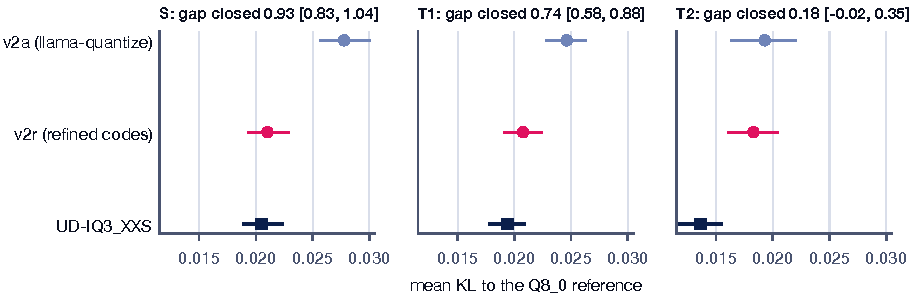
\includegraphics[width=\linewidth]{fig/transfer.pdf}
\caption{Mean KL of v2a, v2r and UD-IQ3\_XXS on S, T1 and T2 with unpaired 95\% chunk intervals. Panel titles give the share of the v2a-to-UD gap that v2r closes, with a paired bootstrap interval.}
\label{fig:transfer}
\end{figure}

The gain is larger on WikiText than on reasoning traces (Table~\ref{tab:v2r}, Figure~\ref{fig:transfer}). On S, the KL difference between v2r and UD-IQ3\_XXS has an interval that includes zero. On T1, held out from the same corpus, v2r closes three quarters of the gap, and the remaining difference from UD has an interval above zero. On T2 it closes less than a fifth. The interval for its difference from v2a includes zero, and its top-1 agreement (95.39\%) falls below v2a's (95.54\%). I estimated the Grams from 51,200 tokens of WikiText-2 training text, a median of about 5,000 tokens per expert for 2,304 input dimensions, so the search fits WikiText's input covariance. UD's encoding keeps its lead off that domain. I registered a follow-up (v2m) before collecting its data (amendment 13). It refines on mixed-domain Grams, including chat-formatted reasoning and tool-use text. The run is still in progress as I write, and its results are outside the scope of this report. The release test for any refined file uses a fresh WikiText span, T3, which I froze before v2r existed and have yet to open. Since v2r has higher KL than UD on T1 with the interval above zero, I expect it to fail on T3 as well. That is an inference until I score T3.

\section{Side results}
\label{sec:side}

\paragraph{A weighted Q2\_0 encoder.} llama.cpp's reference Q2\_0 encoder sets the block scale from the largest weight, which leaves one of the four levels unused, and ignores the importance matrix. My encoder searches signed scales over all four levels and refits each block's scale by importance-weighted least squares (\code{scripts/q2opt.py}). It lowers the mean relative weight error of the down projections from 0.5198 to 0.1354 over 24 layers while keeping the same format, kernels and byte count. I used it in the map for the IQ3\_XXS / Q2\_0 (mine) level, where it still costs more than the larger IQ4\_NL down (B1 0.01201 against 0.00529). Two of the four selection picks used it on B1. v1 used IQ4\_NL for down in B1.

\paragraph{A Metal NVFP4 kernel check.} I also tested a proposed Metal kernel for NVFP4 matrix multiplication end to end. With it, all 20 NVFP4 down tensors of UD-IQ3\_XXS load on the GPU, and the mean KL on S moves by only +0.000079. The registered rule also required every chunk to agree within 2e-4, and 8 of 16 did not, so the check failed as registered. I set the rule without a measured floor for a change of compute path. One untested explanation is that the CPU path multiplies NVFP4 against activations quantized to Q8\_0 while Metal uses f16 and f32. I plan to measure that floor before opening a pull request.

\section{Related work}

LoopQ~\citep{loopq} quantizes weights and activations of looped language models and identifies recursive error accumulation as one source of degradation. \citet{feedback} quantizes a recurrent-depth model and gets better results with Hessians summed over recurrence steps than with one-step Hessians. Each perturbation there applies to all steps, with no single-step condition, no mixture of experts and no GGUF. \citet{tiltedbowl} compare fixed and fresh rounding noise across looped model families. They find that a fixed error does not accumulate when the loop settles, and give the final loops higher precision. Loopy~\citep{loopy} picks a shared low-bit representation by final loss at the deployment depth, because rankings change with depth. LoopQuant~\citep{loopquant} allocates activation precision per loop with Shapley-style marginals and fits per-loop gains on frozen weights. Its pairwise term flags loops whose joint damage exceeds the sum of their individual effects, which is the closest published analogue of the additivity test here. Dory~\citep{dory} is a looped model whose NVFP4 and GGUF releases came from quantization-aware distillation at matched loop counts. The noise controls follow the linearity theorem of \citet{linearity}. Like GPTQ~\citep{gptq} and QuIP~\citep{quip}, my code refinement uses second-order input statistics. The refinement itself is closest to MACaQ~\citep{macaq}.

I apply the same quantized expert block to one pass at a time in a released mixture-of-experts model and compare the sum of the single-pass changes with the all-pass change. The layer-split control gives me the same comparison for parts that share no weights.

\section{Limits}

\begin{itemize}
\item This is an exploratory pilot, and none of it is confirmatory evidence for the thesis.
\item The main results are limited to one machine, one engine commit, one Q8\_0 reference, one importance matrix and these documents at $P = 3$. Absolute KL here is not comparable with numbers on other repositories' cards.
\item I use KL to measure agreement with the reference. Looped models can keep perplexity and still fail on tasks, and I report no task scores.
\item The per-pass test covers B2 at two levels and B3 at one, with each block tested alone. I did not test the whole core at once. The 2-bit level uses stock Q2\_0 down with a relative weight error of about 0.52, so its numbers hold at that amplitude only.
\item The intervals cover only chunk sampling. They give no estimate of variation across seeds, documents or builds. The noise conditions use three draws, and the nine tied-to-independent ratios reuse those draws, so they are not nine independent replications. T2 has five chunks and a coarse bootstrap.
\item The release comparison after the FAIL is post hoc, and the speed figures hold for one Mac and stock llama.cpp.
\item v2r's results on S, T1 and T2 are descriptive, since I had seen all three sets. The refiner still needs review before I use it for a release.
\end{itemize}

\section{Next steps}

I plan three registered tests for the thesis. First, I will replay the base router's choices to separate router flips from smooth nonlinearity as sources of the residual. Second, I will multiply one block's scales by a constant to isolate attenuation in a byte edit that introduces no other error. I will do this in a looped and a non-looped layer at several pass counts to test whether gain error compounds per visit and whether noise does. Third, I will compare two allocators at matched size, one that prices looped bits per visit with a measured surcharge and one that prices them once. With v2m, I am testing whether mixed-domain calibration improves transfer beyond WikiText.

\section*{Reproduction}

The scripts rebuild the model files, data and logs, which are absent from the repository, and resume from where they stopped. The pinned inputs are the model at revision \nolinkurl{ed40e7da625f594fc9c4990f5f66be24873c22d7}, UD-IQ3\_XXS at \nolinkurl{ea0c79b2ecd73669e774c8519b79bfabfddbc027}, the importance matrix from \code{ggml-org/Inkling-2-Mini-GGUF} at \nolinkurl{db61c5b492a6a034d986328d28274af0a439aa6c}, and llama.cpp \nolinkurl{29b52d398b294509746ec0a3f28948a3107c0213}~\citep{llamacpp} plus the seven patches in \code{patches/llama.cpp/}. \code{sh scripts/build-llama.sh} builds the engine and runs the loop tests. The README lists the run scripts in order. I generated the figures with \code{paper/figures.py}, which reads only \code{results/pilot/}.

\bibliographystyle{plainnat}
\bibliography{refs}

\end{document}
